\chapter{Metodogía}
\section{Requerimientos}
El proyecto de gestión de parqueaderos basado en el principio de economía colaborativa deberá contar con una serie de especificaciones y requisitos para su correcto desarrollo e implementación, para comenzar será una aplicación desarrollada en entorno web para su fácil acceso desde cualquier dispositivo y esta deberá contar con la posibilidad de creación y manejo de cuentas personales para la administración de sus objetos vinculados ya sean automóviles o parqueaderos como tal permitiendo añadir estos, de igual manera permitirá modificar la tarifa que desea manejar el usuario y medios de pago, cada automóvil registrado deberá contar con modelo y número de placa y cada parqueadero con la ubicación, número de plazas disponibles, y si es abierto o cerrado.
\\
\\
Se deberá poder consultar en un mapa la ubicación de los parqueaderos registrados disponibles y poder consultar la tarifa que manejan estos  y los medios de pago disponibles, por ende este mapa debe estar actualizado a tiempo real.

\newpage

\section{Proceso de Software}

\begin{figure}[h!]
	\centering
	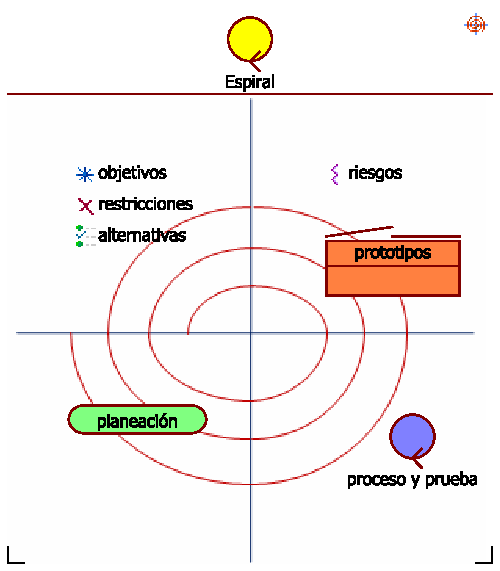
\includegraphics[width=0.7\linewidth]{imgs/espiral}
	\caption[Espiral]{Proceso Espiral}
\end{figure}
